\documentclass{article}
\usepackage{silence}
\WarningFilter{latex}{Writing}
\usepackage{standalone}
\usepackage{tikz}
\usetikzlibrary{
  matrix,
  calc,
  positioning,
  arrows,
  intersections,
  math,
  external}
\usepackage{pgfplots}
  \usepgfplotslibrary{external}
  \pgfplotsset{compat=1.18}
\usepackage{ifthen}
\usepackage{amssymb}
\usepackage{currfile}
\usepackage{etoolbox}

\tikzexternalize[prefix=./]
\tikzsetfigurename{figure-}
\newcommand*\setmyname{%
  \expandafter\tikzsetfigurename\expandafter{\currfilebase-}%
}
\makeatletter
\apptocmd{\sa@document}{\setmyname}{\typeout{Append to document: OK!}}{\typeout{Append to document: Oh, no!}}
\makeatother

%%% PLOTS %%%
\begin{filecontents*}[overwrite]{plot.tex}
\documentclass[tikz]{standalone}
\usepackage{pgfplots}
  \usetikzlibrary{positioning}
  \usepgfplotslibrary{external}
  \pgfplotsset{
    % width=10cm,
    compat=1.18
  }
\begin{document}

%% PWISE MULS -- SINGLE SLICE%%
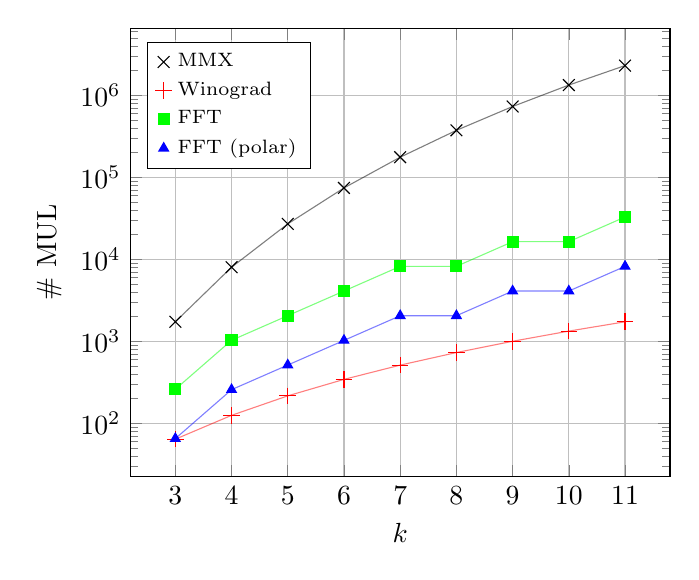
\begin{tikzpicture}
  \begin{semilogyaxis}[
    domain=3:11,
    xtick={3,...,11},
    % y domain=3:11, 
    grid=major,
    xlabel={$k$},
    ylabel={\# MUL},
    legend style={font=\scriptsize},
    legend cell align=left,
    legend pos=north west,
    scatter/classes={
      a={mark=square*, blue},
      b={mark=square*, red},
      c={mark=square, black},
      d={mark=triangle*, blue},
      e={mark=triangle*, red},
      f={mark=triangle*, black},
      g={mark=x, black},
      h={mark= diamond*, pink}
    },
  ]
    % MMX
    \addplot[
      samples=9,
      draw opacity=0.5,
      color=black,
    ]{
      ((2+x-1)^3)*(x^3)
    };
    \addplot[
      mark=x,
      mark size=3pt,
      samples=9,
      only marks,
      color=black,
      draw opacity=1,
    ]{
      ((2+x-1)^3)*(x^3)
    };

    % WINOGRAD
    \addplot[
      samples=9,
      draw opacity=0.5,
      color=red,
    ]{
      ((2+x-1)^3)
    };
    \addplot[
      mark=+,
      mark size=3pt,
      samples=9,
      only marks,
      color=red,
      draw opacity=1,
    ]{
      ((2+x-1)^3)
    };

    % FFT (rec)
    \addplot[
      samples=9,
      draw opacity=0.5,
      color=green,
    ]{
      4*((pow(2,ceil(log2((2*x-1)^3)))/2)+1)
    };
    \addplot[
      mark=square*,
      mark size=2pt, 
      samples=9,
      only marks,
      color=green,
      draw opacity=1,
    ]{
      4*((pow(2,ceil(log2((2*x-1)^3)))/2)+1)
    };

    % FFT (polar)
    \addplot[
      samples=9,
      draw opacity=0.5,
      color=blue,
    ]{
      (pow(2,ceil(log2((2*x-1)^3)))/2)+1
    };
    \addplot[
      mark=triangle*,
      mark size=2pt, 
      samples=9,
      only marks,
      color=blue,
      draw opacity=1,
    ]{
      (pow(2,ceil(log2((2*x-1)^3)))/2)+1
    };
  \legend{,MMX,,Winograd,,FFT,,FFT (polar)}
  \end{semilogyaxis}
\end{tikzpicture}

%% PWISE MULS -- FULL%% 
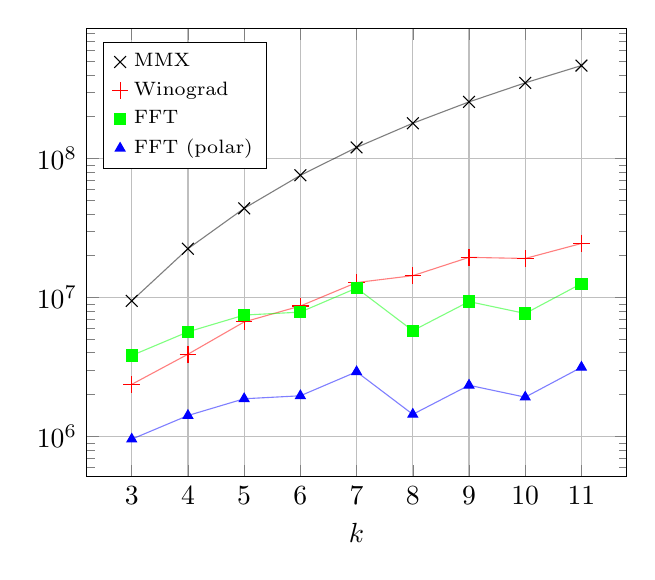
\begin{tikzpicture}
  \begin{semilogyaxis}[
    domain=3:11,
    xtick={3,...,11},
    % y domain=3:11, 
    grid=major,
    xlabel={$k$},
    ylabel={},
    legend style={font=\scriptsize},
    legend cell align=left,
    legend pos=north west,
  ]
    % MMX
    \addplot[
      samples=9,
      draw opacity=0.5,
      color=black,
    ]{
      (128)*(171)*(16)*(x^3)
    };
    \addplot[
      mark=x,
      mark size=3pt,
      samples=9,
      only marks,
      color=black,
      draw opacity=1,
    ]{
      (128)*(171)*(16)*(x^3)
    };

    % WINOGRAD
    \addplot[
      samples=9,
      draw opacity=0.5,
      color=red,
    ]{
      ceil((128-x)/2)*
      ceil((171-x)/2)*
      ceil((16-x)/2)*
      ((2+x-1)^3)
    };
    \addplot[
      mark=+,
      mark size=3pt,
      samples=9,
      only marks,
      color=red,
      draw opacity=1,
    ]{
      ceil((128-x)/2)*
      ceil((171-x)/2)*
      ceil((16-x)/2)*
      ((2+x-1)^3)
    };

    % FFT (rec)
    \addplot[
      samples=9,
      draw opacity=0.5,
      color=green,
    ]{
      4*ceil(128/x)*ceil(171/x)*ceil(16/x)*
      ((pow(2,ceil(log2((2*x-1)^3)))/2)+1)
    };
    \addplot[
      mark=square*,
      mark size=2pt,
      samples=9,
      only marks,
      color=green,
      draw opacity=1,
    ]{
      4*ceil(128/x)*ceil(171/x)*ceil(16/x)*
      ((pow(2,ceil(log2((2*x-1)^3)))/2)+1)
    };

    % FFT (polar)
    \addplot[
      samples=9,
      draw opacity=0.5,
      color=blue,
    ]{
      ceil(128/x)*ceil(171/x)*ceil(16/x)*
      ((pow(2,ceil(log2((2*x-1)^3)))/2)+1)
    };
    \addplot[
      mark=triangle*,
      mark size=2pt,
      samples=9,
      only marks,
      color=blue,
      draw opacity=1,
    ]{
      ceil(128/x)*ceil(171/x)*ceil(16/x)*
      ((pow(2,ceil(log2((2*x-1)^3)))/2)+1)
    };
  \legend{,MMX,,Winograd,,FFT,,FFT (polar)}
  \end{semilogyaxis}
\end{tikzpicture}

\end{document}
\end{filecontents*}

%%% MATRIX %%%
\begin{filecontents*}[overwrite]{matrix.tex}
\documentclass[tikz]{standalone}
\begin{document}
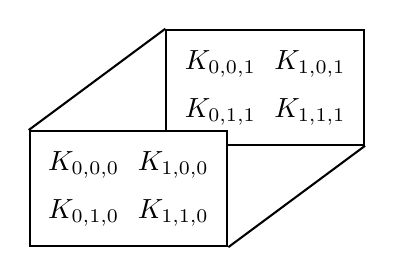
\begin{tikzpicture}[
  >=stealth,
  line width=0.75pt,
  every node/.style={anchor=north east,fill=white,minimum width=1.1cm,minimum height=6mm},
  ampersand replacement=\&
]%
  \matrix (mA) [draw,matrix of math nodes]
  {
    K_{0,0,1} \& K_{1,0,1} \\
    K_{0,1,1} \& K_{1,1,1} \\
  };

  \matrix (mB) [draw,matrix of math nodes] at ($(mA.south west)+(0.8,0.2)$)
  {
    K_{0,0,0} \& K_{1,0,0} \\
    K_{0,1,0} \& K_{1,1,0} \\
  };
  \draw(mA.north west)--(mB.north west);
  \draw(mA.south east)--(mB.south east);
\end{tikzpicture}
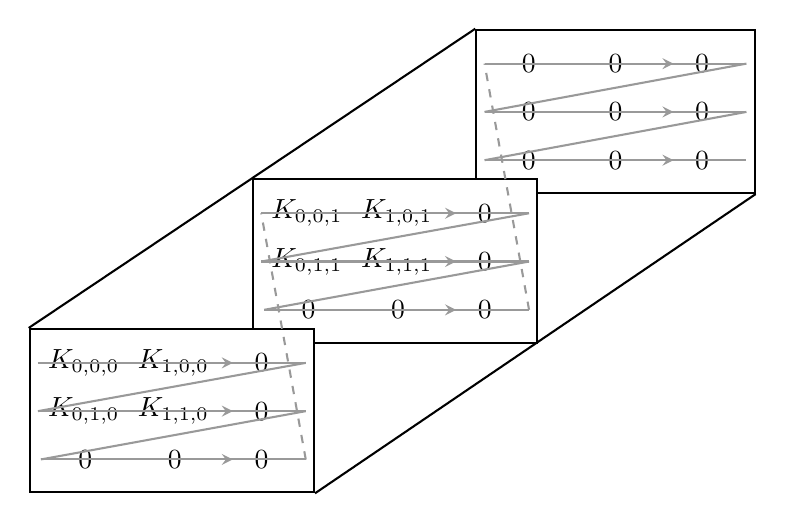
\begin{tikzpicture}[
  >=stealth,
  line width=0.75pt,
  every node/.style={anchor=north east,fill=white,minimum width=1.1cm,minimum height=6mm},
  ampersand replacement=\&
]%
  \matrix (mA) [draw,matrix of math nodes]
  {
    |(mA1)| 0 \& 0 \& |(mA2)| 0 \\
    |(mA3)| 0 \& 0 \& |(mA4)| 0 \\
    |(mA5)| 0 \& 0 \& |(mA6)| 0 \\
  };

  \matrix (mB) [draw,matrix of math nodes] at ($(mA.south west)+(0.8,0.2)$)
  {
    |(mB1)| K_{0,0,1} \& K_{1,0,1} \& |(mB2)| 0 \\
    |(mB3)| K_{0,1,1} \& K_{1,1,1} \& |(mB4)| 0 \\
    |(mB5)| 0         \& 0         \& |(mB6)| 0 \\
  };

  \matrix (mC) [draw,matrix of math nodes] at ($(mB.south west)+(0.8,0.2)$)
  {
    |(mC1)| K_{0,0,0} \& K_{1,0,0} \& |(mC2)| 0 \\
    |(mC3)| K_{0,1,0} \& K_{1,1,0} \& |(mC4)| 0 \\
    |(mC5)| 0         \& 0         \& |(mC6)| 0 \\
  };

  \draw(mA.north west)--(mC.north west);
  \draw(mA.south east)--(mC.south east);

  \draw[->,color=black!40]     (mC1.west) -- ($(mC2.west)+(0.2,0)$);
  \draw[color=black!40]        (mC2.west) -- (mC2.east);
  \draw[color=black!40]        (mC2.east) -- (mC3.west);
  \draw[->,color=black!40]     (mC3.west) -- ($(mC4.west)+(0.2,0)$);
  \draw[color=black!40]        (mC4.west) -- (mC4.east);
  \draw[color=black!40]        (mC4.east) -- (mC5.west);
  \draw[->,color=black!40]     (mC5.west) -- ($(mC6.west)+(0.2,0)$);
  \draw[color=black!40]        (mC6.west) -- (mC6.east);
  \draw[dashed,color=black!40] (mC6.east) -- (mB1.west);

  \draw[->,color=black!40]     (mB1.west) -- ($(mB2.west)+(0.2,0)$);
  \draw[color=black!40]        (mB2.west) -- (mB2.east);
  \draw[color=black!40]        (mB2.east) -- (mB3.west);
  \draw[->,color=black!40]     (mB3.west) -- ($(mB4.west)+(0.2,0)$);
  \draw[color=black!40]        (mB4.west) -- (mB4.east);
  \draw[color=black!40]        (mB4.east) -- (mB5.west);
  \draw[->,color=black!40]     (mB5.west) -- ($(mB6.west)+(0.2,0)$);
  \draw[color=black!40]        (mB6.west) -- (mB6.east);
  \draw[dashed,color=black!40] (mB6.east) -- (mA1.west);

  \draw[->,color=black!40]     (mA1.west) -- ($(mA2.west)+(0.2,0)$);
  \draw[color=black!40]        (mA2.west) -- (mA2.east);
  \draw[color=black!40]        (mA2.east) -- (mA3.west);
  \draw[->,color=black!40]     (mA3.west) -- ($(mA4.west)+(0.2,0)$);
  \draw[color=black!40]        (mA4.west) -- (mA4.east);
  \draw[color=black!40]        (mA4.east) -- (mA5.west);
  \draw[->,color=black!40]     (mA5.west) -- ($(mA6.west)+(0.2,0)$);
  \draw[color=black!40]        (mA6.west) -- (mA6.east);

\end{tikzpicture}
\end{document}
\end{filecontents*}

%%% UNIT CIRCLE %%%
\begin{filecontents*}[overwrite]{unit_circle.tex}
\documentclass[tikz]{standalone}
\begin{document}
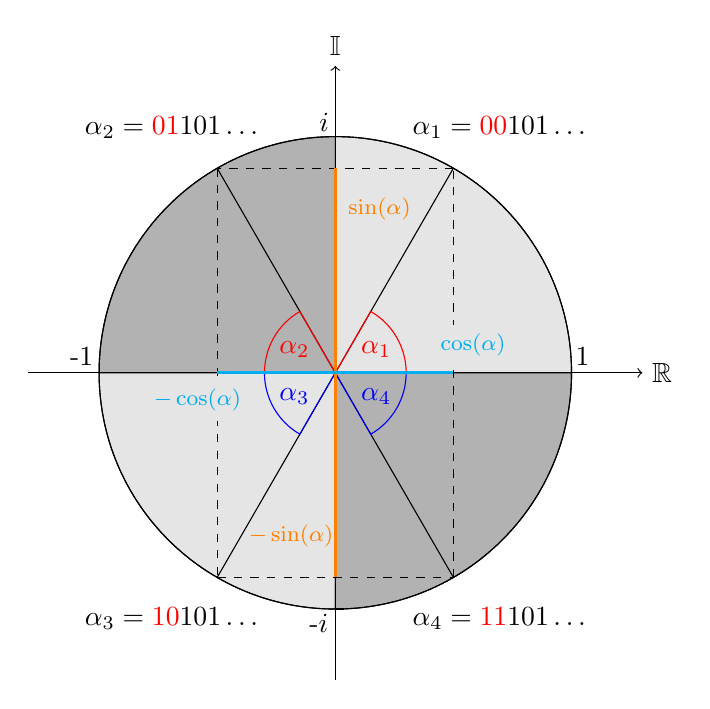
\begin{tikzpicture}[
  scale=3
]%
  % Quadrants
  \filldraw[fill=gray!20,draw]
    (0,0) -- (1 cm,0pt) arc [start angle=0, end angle=90, radius=1cm] -- cycle;
  \filldraw[fill=gray!60,draw]
    (0,0) -- (0pt,1 cm) arc [start angle=90, end angle=180, radius=1cm] -- cycle;
  \filldraw[fill=gray!20,draw]
    (0,0) -- (-1 cm,0pt) arc [start angle=180, end angle=270, radius=1cm] -- cycle;
  \filldraw[fill=gray!60,draw]
    (0,0) -- (0pt,- 1cm) arc [start angle=270, end angle=360, radius=1cm] -- cycle;

  % Unit circle and lines
  \path [name path=unit circle,draw] (0,0) circle [radius=1cm];
  \path [name path=q1 line,draw] (0,0) -- (60:1.0cm);
  \path [name path=q2 line,draw] (0,0) -- (120:1.0cm);
  \path [name path=q3 line,draw] (0,0) -- (240:1.0cm);
  \path [name path=q4 line,draw] (0,0) -- (300:1.0cm);

  % Grid and coordinate plane
  % \draw[step=.5cm,gray,very thin] (-1.2,-1.2) grid (1.2,1.2);
  \draw[->] (-1.3,0) -- (1.3,0) coordinate (x axis)node[right]{$\mathbb{R}$};
  \draw[->] (0,-1.3) -- (0,1.3) coordinate (y axis)node[above]{$\mathbb{I}$};
  \draw (1 cm,1pt) -- (1 cm,0pt) node[anchor=east,xshift=10pt,yshift=6pt] {$1$};
  \draw (-1 cm,1pt) -- (-1 cm,0pt) node[anchor=west,xshift=-14pt,yshift=6pt] {-$1$};
  \draw (1pt,1 cm) -- (0pt, 1 cm) node[anchor=north,xshift=-4pt,yshift=12pt] {$i$};
  \draw (1pt,-1 cm) -- (0pt, -1 cm) node[anchor=south,xshift=-6pt,yshift=-12pt] {-$i$};

  % Angles
  \path[draw=red]
    (0,0) -- (3mm,0mm) arc [start angle=0, end angle=60, radius=3mm] -- cycle;
  \node[red] at (30:2mm) {$\alpha_1$};

  \path[draw=red]
    (0,0) -- (-3mm,0mm) arc [start angle=180, end angle=120, radius=3mm] -- cycle;
  \node[red] at (150:2mm) {$\alpha_2$};

  \path[draw=blue]
    (0,0) -- (-3mm,0mm) arc [start angle=180, end angle=240, radius=3mm] -- cycle;
  \node[blue] at (210:2mm) {$\alpha_3$};

  \path[draw=blue]
    (0,0) -- (3mm,0mm) arc [start angle=0, end angle=-60, radius=3mm] -- cycle;
  \node[blue] at (-30:2mm) {$\alpha_4$};

  % Reflections
  \path [name intersections={of=unit circle and q1 line, by=q1inter}] (0,0);
  \path [name intersections={of=unit circle and q2 line, by=q2inter}] (0,0);
  \path [name intersections={of=unit circle and q3 line, by=q3inter}] (0,0);
  \path [name intersections={of=unit circle and q4 line, by=q4inter}] (0,0);

  \draw [dashed] (q1inter) -- (q2inter);
  \draw [dashed] (q2inter) -- (q3inter);
  \draw [dashed] (q3inter) -- (q4inter);
  \draw [dashed] (q4inter) -- (q1inter);

  % Sines and cosines
  \draw[very thick,orange]
    (0,0) -- node[above,xshift=16pt,yshift=0.5cm] {\footnotesize$\sin(\alpha)$} (y axis |- 60:1cm);
  \draw[very thick,orange]
    (0:0) -- node[below,xshift=-16pt,yshift=-0.5cm] {\footnotesize$-\sin(\alpha)$} (y axis |- 240:1cm);
  \draw[very thick,cyan]
    (0,0) -- node[above,xshift=1cm,yshift=2pt,fill=gray!20] {\footnotesize$\cos(\alpha)$} (60:1cm |- x axis);
  \draw[very thick,cyan]
    (0,0) -- node[below,xshift=-1cm,yshift=-2pt,fill=gray!20] {\footnotesize$-\cos(\alpha)$} (120:1cm |- x axis);

  % Angle descriptions
  \node[xshift=8pt] at (60:1.2 cm) {$\alpha_1 = \textcolor{red}{00}101\ldots$};
  \node[xshift=-8pt] at (120:1.2 cm) {$\alpha_2 = \textcolor{red}{01}101\ldots$};
  \node[xshift=-8pt] at (240:1.2 cm) {$\alpha_3 = \textcolor{red}{10}101\ldots$};
  \node[xshift=8pt] at (300:1.2 cm) {$\alpha_4 = \textcolor{red}{11}101\ldots$};

  % Rotated version
  % \node[rotate=-30,xshift=8pt] at (60:1.2 cm) {$\alpha_1 = \textcolor{red}{00}101\ldots$};
  % \node[rotate=30,xshift=-8pt] at (120:1.2 cm) {$\alpha_2 = \textcolor{red}{01}101\ldots$};
  % \node[rotate=-30,xshift=-8pt] at (240:1.2 cm) {$\alpha_3 = \textcolor{red}{10}101\ldots$};
  % \node[rotate=30,xshift=8pt] at (300:1.2 cm) {$\alpha_4 = \textcolor{red}{11}101\ldots$};
\end{tikzpicture}
\end{document}
\end{filecontents*}

%%% FFT %%%
\begin{filecontents*}[overwrite]{fft.tex}
\documentclass[tikz]{standalone}
\begin{document}
\pgfkeys{/pgf/number format/.cd,fixed,precision=2}
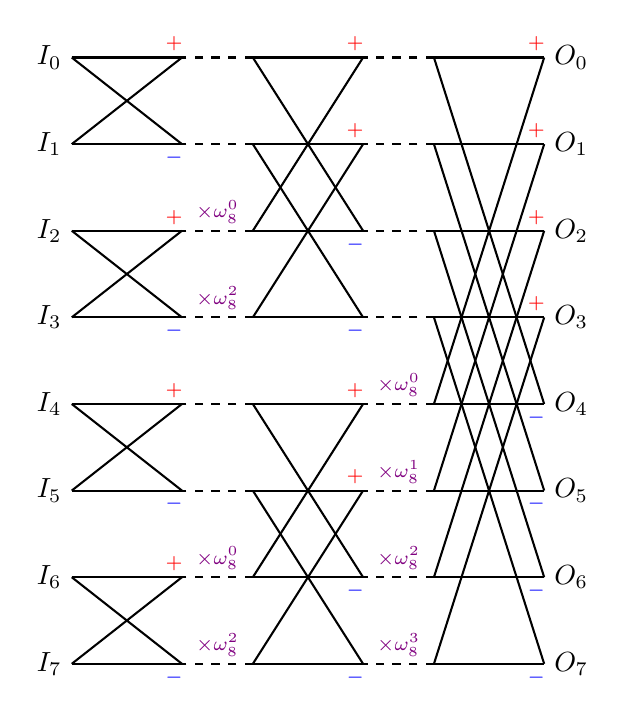
\begin{tikzpicture}[
  % circuit ee IEC,
  >=stealth,
  line width=0.75pt
]%
  \tikzmath{
    \bx = 1.4;      % butterfly width
    \by = -1.1;     % butterfly height
    \sx = 0.9;      % space between stages
    \N  = 8;        % number of points
    \bn = \N/2-1;   % number of butterflies -1
    \sn = ceil{log2(\N)}-1; % number of stages -1 
  }

  \foreach \s in {0,...,\sn} {
    \foreach \b in {0,...,\bn} {
      \tikzmath{
        \gs  = 2^\s;            % group size
        \bg  = mod(\b,\gs);     % butterfly group pos
        \bxp = \sx*\s + \bx*\s; % butterfly x pos
        \byp = 2*\by*\b;        % butterfly y pos
        \w   = int(mod(\b,pow(2,\s)) * pow(2,\sn-\s)); % twiddle factor
        \i1  = int(2*\b);       % input index top
        \i2  = int(2*\b+1);     % input index bot
      }
      % Inputs/Outputs
      \ifthenelse{\s=0}{
        \node[left] at (\bxp cm, \byp cm) {$I_{\i1}$};
        \node[left] at (\bxp cm, \byp cm + \by cm) {$I_{\i2}$};
      }{}
      \ifthenelse{\s=\sn}{
        \node[right] at (\bxp cm + \bx cm, \byp cm) {$O_{\i1}$};
        \node[right] at (\bxp cm + \bx cm, \byp cm + \by cm) {$O_{\i2}$};
      }{}

      % Bfly top and bottom
      \draw  (\bxp cm,          \byp cm)
          -- (\bxp cm + \bx cm, \byp cm) 
             (\bxp cm,          \byp cm + \by cm)
          -- (\bxp cm + \bx cm, \byp cm + \by cm)  ;

      % Bfly diagonals
      \draw  (\bxp cm,          \byp cm - \by*\bg cm)
          -- (\bxp cm + \bx cm, \byp cm - \by*\bg cm + \by*\gs cm)
              node[text=blue, below, xshift=-0.1cm, yshift=0.05cm] {\scriptsize$-$}
             (\bxp cm,          \byp cm - \by*\bg cm + \by*\gs cm)
          -- (\bxp cm + \bx cm, \byp cm - \by*\bg cm)
              node[text=red, above, xshift=-0.1cm, yshift=-0.05cm] {\scriptsize$+$};

      \ifthenelse{\not{\s=0}}{
      % Connection grid
      \draw [dashed]
           (\bxp cm,          \byp cm)
        -- (\bxp cm - \sx cm, \byp cm)
           (\bxp cm,          \byp cm + \by cm)
        -- (\bxp cm - \sx cm, \byp cm + \by cm);

      % Twiddle-factor mult
      \path (\bxp cm         , \byp cm - \by*\bg cm + \by*\gs cm)
        --    node[above, yshift=-1]
                {\textcolor{violet}{\scriptsize{$\times\omega^{\w}_{\N}$}}}
            (\bxp cm - \sx cm, \byp cm - \by*\bg cm + \by*\gs cm);
      }{}
    }
  }
  % \pgfmathparse{equal(mod(\bg,2), 0)}
  % \ifthenelse{\pgfmathresult = 1}{
  % \draw (\bx*\s cm + \bx cm,          \byp cm - \by*\bg cm) to [resistor]
  %       (\bx*\s cm + \bx cm + \sx cm, \byp cm - \by*\bg cm);
\end{tikzpicture}
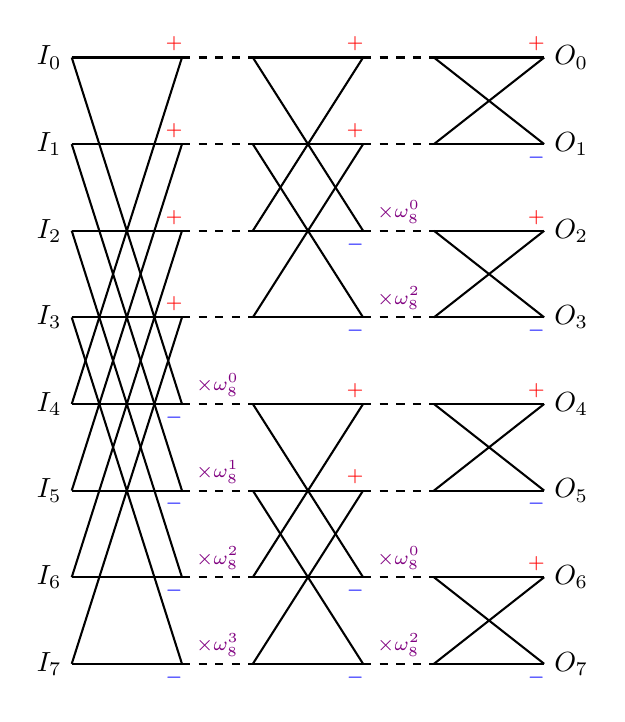
\begin{tikzpicture}[
  % circuit ee IEC,
  >=stealth,
  line width=0.75pt
]%
  \tikzmath{
    \bx = 1.4;      % butterfly width
    \by = -1.1;     % butterfly height
    \sx = 0.9;      % space between stages
    \N  = 8;        % number of points
    \bn = \N/2-1;   % number of butterflies -1
    \sn = ceil{log2(\N)}-1; % number of stages -1 
  }

  \foreach \s in {0,...,\sn} {
    \foreach \b in {0,...,\bn} {
      \tikzmath{
        \gs  = 2^(\sn-\s);      % group size
        \bg  = mod(\b,\gs);     % butterfly group pos
        \bxp = \sx*\s + \bx*\s; % butterfly x pos
        \byp = 2*\by*\b;        % butterfly y pos
        \w   = int(mod(\b,pow(2,\sn-\s)) * pow(2,\s)); % twiddle factor
        \i1  = int(2*\b);       % input index top
        \i2  = int(2*\b+1);     % input index bot
      }
      % Inputs/Outputs
      \ifthenelse{\s=0}{
        \node[left] at (\bxp cm, \byp cm) {$I_{\i1}$};
        \node[left] at (\bxp cm, \byp cm + \by cm) {$I_{\i2}$};
      }{}
      \ifthenelse{\s=\sn}{
        \node[right] at (\bxp cm + \bx cm, \byp cm) {$O_{\i1}$};
        \node[right] at (\bxp cm + \bx cm, \byp cm + \by cm) {$O_{\i2}$};
      }{}

      % Bfly top and bottom
      \draw  (\bxp cm,          \byp cm)
          -- (\bxp cm + \bx cm, \byp cm) 
             (\bxp cm,          \byp cm + \by cm)
          -- (\bxp cm + \bx cm, \byp cm + \by cm)  ;

      % Bfly diagonals
      \draw  (\bxp cm,          \byp cm - \by*\bg cm)
          -- (\bxp cm + \bx cm, \byp cm - \by*\bg cm + \by*\gs cm)
              node[text=blue, below, xshift=-0.1cm, yshift=0.05cm] {\scriptsize$-$}
             (\bxp cm,          \byp cm - \by*\bg cm + \by*\gs cm)
          -- (\bxp cm + \bx cm, \byp cm - \by*\bg cm)
              node[text=red, above, xshift=-0.1cm, yshift=-0.05cm] {\scriptsize$+$};

      \ifthenelse{\not{\s=\sn}}{
      % Connection grid
      \draw [dashed]
           (\bxp cm + \bx cm,          \byp cm)
        -- (\bxp cm + \bx cm + \sx cm, \byp cm)
           (\bxp cm + \bx cm,          \byp cm + \by cm)
        -- (\bxp cm + \bx cm + \sx cm, \byp cm + \by cm);

      % Twiddle-factor mult
      \path (\bxp cm + \bx cm,          \byp cm - \by*\bg cm + \by*\gs cm)
        --    node[above, yshift=-1]
                {\textcolor{violet}{\scriptsize{$\times\omega^{\w}_{\N}$}}}
            (\bxp cm + \bx cm + \sx cm, \byp cm - \by*\bg cm + \by*\gs cm);
      }{}
    }
  }
  % \pgfmathparse{equal(mod(\bg,2), 0)}
  % \ifthenelse{\pgfmathresult = 1}{
  % \draw (\bx*\s cm + \bx cm,          \byp cm - \by*\bg cm) to [resistor]
  %       (\bx*\s cm + \bx cm + \sx cm, \byp cm - \by*\bg cm);
\end{tikzpicture}
\end{document}
\end{filecontents*}

%%% PIPELINE %%%
\begin{filecontents*}[overwrite]{pipeline.tex}
\documentclass[tikz]{standalone}
\begin{document}
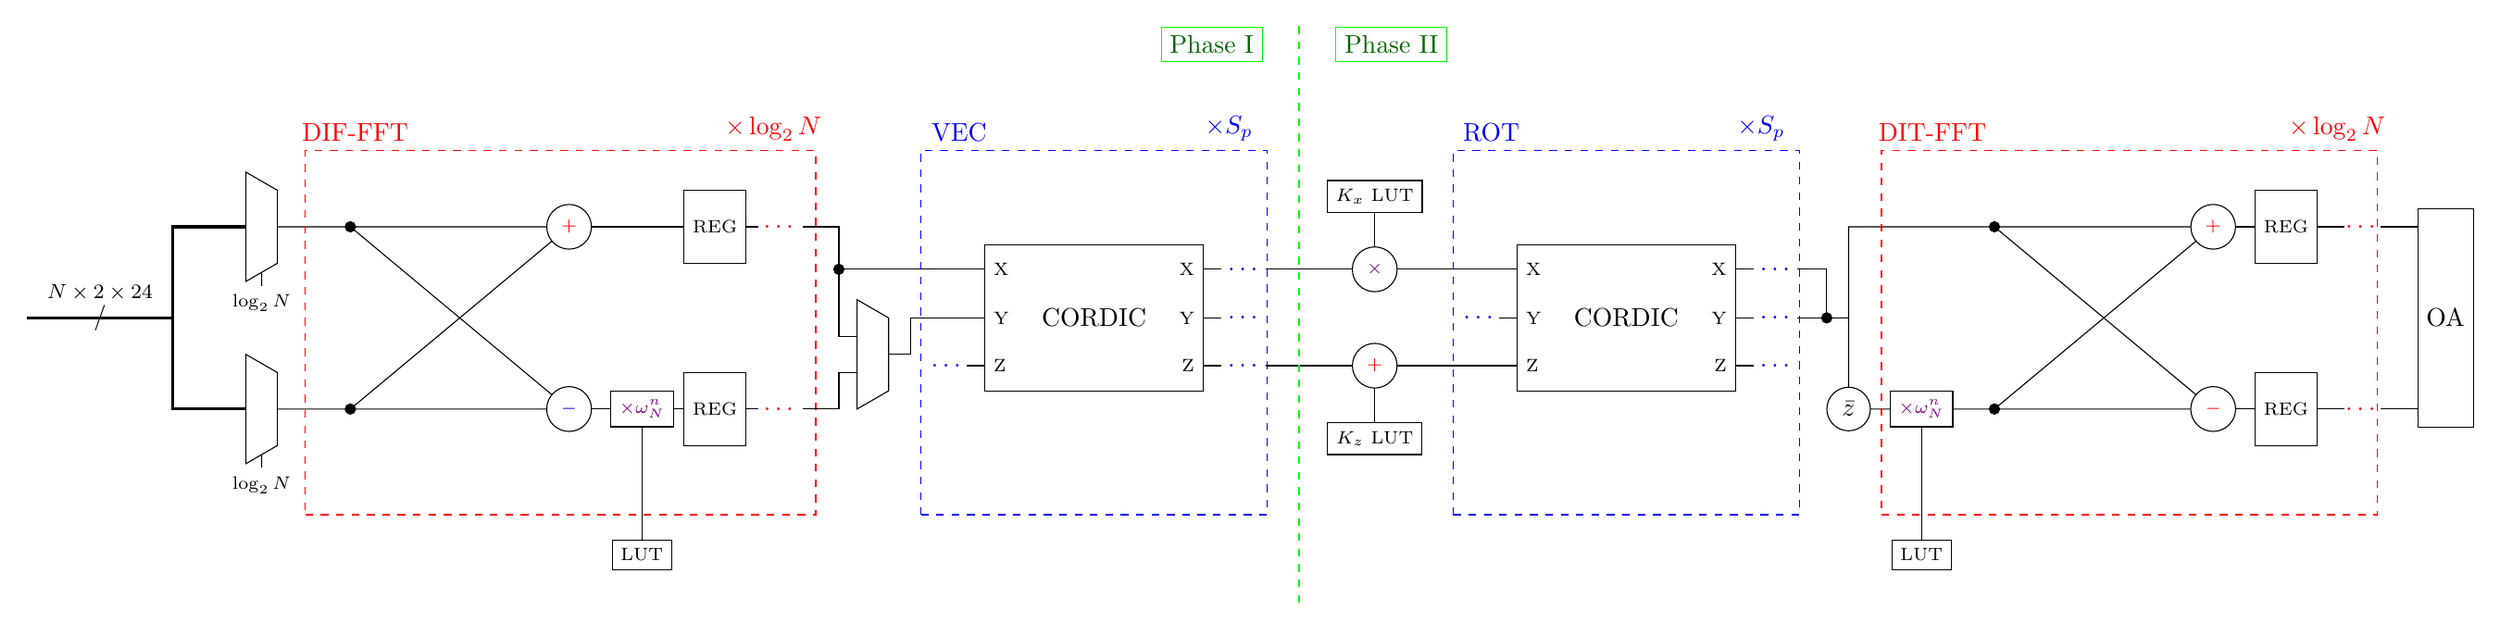
\begin{tikzpicture}%
  % Input bus
  \draw [very thick]
    (1,0) --
    node{/}
    node[above,yshift=1mm]{\footnotesize{$N \times 2 \times 24$}}
    (3,0) coordinate (bin)
    (bin) --++ (90:1.25) --++ (0:1)
    (bin) --++ (90:-1.25) --++ (0:1);

  % FFT MUXes
  \draw 
    (4,0.5)   coordinate (FMUXO1)--++
    (90:1.5)  coordinate (FMUXA1)--++
    (-30:0.5) coordinate (FMUXB1)--++
    (-90:1)   coordinate (FMUXC1)--
    cycle
    (4,-0.5)  coordinate (FMUXO2)--++ 
    (-90:1.5) coordinate (FMUXA2)--++
    (30:0.5)  coordinate (FMUXB2)--++
    (90:1)    coordinate (FMUXC2)--
    cycle
    ($(FMUXB1)!0.5!(FMUXC1)$) coordinate (muxout0)--++
      (0:1) coordinate (bfly0)
    ($(FMUXC2)!0.5!(FMUXB2)$) coordinate (muxout1)--++
      (0:1) coordinate (bfly1)
    ($(FMUXO1)!0.5!(FMUXC1)$)
      node[below,yshift=-5,fill=white]{\scriptsize{$\log_{2}N$}}--++
      (-90:0.4)
    ($(FMUXA2)!0.5!(FMUXB2)$)
      node[below,yshift=-5,fill=white]{\scriptsize{$\log_{2}N$}}--++
      (-90:0.4);

  % FFT Butterfly
  \draw
    (bfly0) --++ (0:3) coordinate (bfly2) 
    (bfly1) --++ (0:3) coordinate (bfly3)
    (bfly0) -- (bfly3)
    (bfly1) -- (bfly2);
  \filldraw
    (bfly0) circle (2pt)
    (bfly1) circle (2pt);
  \draw 
    (bfly2) --++ (0:2) coordinate (bout1)
    (bfly3) --++ (0:2) coordinate (bout2);
  \node[text=red,circle,draw,fill=white] at (bfly2) {\scriptsize$+$};
  \node[text=blue,circle,draw,fill=white] at (bfly3) {\scriptsize$-$};

  % FFT Wmul
  \draw ($(bfly3)!0.5!(bout2)$) --++ (-90:2)
    node[rectangle,draw,fill=white] {\scriptsize{LUT}};
  \node[rectangle,draw,fill=white] at ($(bfly3)!0.5!(bout2)$)
    {\textcolor{violet}{\scriptsize{$\times\omega^{n}_{N}$}}};

  % FFT Registers
  \draw
    (bout1) --++ (0:0.6) coordinate (recursion1)
    (bout2) --++ (0:0.6) coordinate (recursion2);
  \node[rectangle,draw,fill=white,minimum height=1cm] at (bout1) {\scriptsize{REG}};
  \node[rectangle,draw,fill=white,minimum height=1cm] at (bout2) {\scriptsize{REG}};
  \path
    (recursion1) --++ (0:0.6) coordinate (cordic1in1)
    (recursion2) --++ (0:0.6) coordinate (cordic1in2);
  \node[text=red] at ($(recursion1)!0.5!(cordic1in1)$) {\dots};
  \node[text=red] at ($(recursion2)!0.5!(cordic1in2)$) {\dots};

  % FFT delimeter
  \path (bout1) -- coordinate (bout0) (bout2);
  \node[
    rectangle,
    draw=red,
    dashed,
    minimum width=7cm,
    minimum height=5cm,
    xshift=1.6cm,
    yshift=-0.2cm]
    at ($(bin)!0.5!(bout0)$) {};
  \node[text=red,above,xshift=2.5cm,yshift=2.3cm] at (bin) {DIF-FFT};
  \node[text=red,above,xshift=0.8cm,yshift=2.3cm] at (bout0) {$\times \log_{2}N$};

  % CORDIC-1 points
  \path
    (bout0) --++ (0:5.2) coordinate (cordic1)
    (cordic1)
      --++ (180:1.5)    coordinate (cordic1yin)
      --++ (90:0.6666)  coordinate (cordic1xin)
      --++ (-90:1.3222) coordinate (cordic1zin)
    (cordic1)
      --++ (0:1.5)      coordinate (cordic1yout)
      --++ (90:0.6666)  coordinate (cordic1xout)
      --++ (-90:1.3222) coordinate (cordic1zout);

  % CORDIC-1 connections  
  \draw
    (cordic1in1) --++ (0:0.5) coordinate (cordic1in1b) --
      (cordic1in1b |- cordic1xin) coordinate (csplit1) -- (cordic1xin)
    (cordic1zin) --++ (180:0.25) node[text=blue,xshift=-0.25cm]{\dots}
    (cordic1xout) --++ (0:0.25) node[text=blue,xshift=0.32cm]{\dots} coordinate (recursion3)
    (cordic1yout) --++ (0:0.25) node[text=blue,xshift=0.32cm]{\dots}
    (cordic1zout) --++ (0:0.25) node[text=blue,xshift=0.32cm]{\dots} coordinate (recursion4);
  \filldraw (csplit1) circle (2pt);

  % CORDIC-1 MUX
  \path (cordic1in2) --++ (0:0.75) coordinate (cmux1);
  \draw 
    (cmux1) --++ 
    (90:1.5)  coordinate (CMUXA1)--++
    (-30:0.5) coordinate (CMUXB1)--++
    (-90:1)   coordinate (CMUXC1)--
    cycle;
  \path (cmux1) --++ (90:0.5) coordinate (cmux1in1) --++ (90:0.5) coordinate (cmux1in2);
  \draw
    (cordic1in2) --++ (0:0.5) --++ (90:0.5) -- (cmux1in1)
    (csplit1) -- (csplit1 |- cmux1in2) -- (cmux1in2)
    ($(CMUXC1)!0.5!(CMUXB1)$) --++ (0:0.3) coordinate (cmux1out)
      -- (cmux1out |- cordic1yin) -- (cordic1yin);

  % CORDIC-1 block
  \node[rectangle,draw,fill=white,minimum width=3cm,minimum height=2cm] at (cordic1) {CORDIC};
  \node[right] at (cordic1xin)  {\scriptsize{X}};
  \node[right] at (cordic1yin)  {\scriptsize{Y}};
  \node[right] at (cordic1zin)  {\scriptsize{Z}};
  \node[left] at (cordic1xout) {\scriptsize{X}};
  \node[left] at (cordic1yout) {\scriptsize{Y}};
  \node[left] at (cordic1zout) {\scriptsize{Z}};

  % CORDIC-1 delimeter
  \node[
    rectangle,
    draw=blue,
    dashed,
    minimum width=4.75cm,
    minimum height=5cm,
    xshift=0cm,
    yshift=-0.2cm]
    at (cordic1) {};
  \node[text=blue,above,xshift=-0.35cm,yshift=2.3cm] at (cordic1yin) {VEC};
  \node[text=blue,above,xshift=0.35cm,yshift=2.3cm] at (cordic1yout) {$\times S_p$};

  % MUL/ADD
  \path
    (recursion3) --++ (0:0.6) coordinate (mul)
    (recursion4) --++ (0:0.6) coordinate (add);
  \draw
    (mul) --++ (0:2) coordinate (cordic2in1)
    (add) --++ (0:2) coordinate (cordic2in2)
    (mul) --++ (0:1.5) coordinate (mul0)
      node[text=violet,circle,draw,fill=white] {\scriptsize$\times$}
    --++ (90:1)
      node[rectangle,draw,fill=white] {\scriptsize{$K_x$ LUT}}
    (add) --++ (0:1.5) coordinate (add0)
      node[text=red,circle,draw,fill=white] {\scriptsize$+$}
    --++ (-90:1)
      node[rectangle,draw,fill=white] {\scriptsize{$K_z$ LUT}};

  % Mirror line
  \path
    (cordic1) --++ (0:4.75/2) coordinate (mirror1)
    ($(mul0)!0.5!(add0)$) --++ (180:0.6) coordinate (mirror2)
    (mirror1) --   coordinate (mirror0) (mirror2)
    (mirror0) --++ (90:4) coordinate (mirror);
  \draw[color=green,dashed]
    (mirror)  --++ (-90:8);
  \node[text=black!60!green,draw=green,left,xshift=-0.5cm,yshift=-0.25cm]
    at (mirror) {Phase I};
  \node[text=black!60!green,draw=green,right,xshift=0.5cm,yshift=-0.25cm]
    at (mirror) {Phase II};

  % CORDIC-2 points
  \path
    (cordic1) --++ (0:7.3) coordinate (cordic2)
    (cordic2)
      --++ (180:1.5)    coordinate (cordic2yin)
      --++ (90:0.6666)  coordinate (cordic2xin)
      --++ (-90:1.3222) coordinate (cordic2zin)
    (cordic2)
      --++ (0:1.5)      coordinate (cordic2yout)
      --++ (90:0.6666)  coordinate (cordic2xout)
      --++ (-90:1.3222) coordinate (cordic2zout);

  % CORDIC-2 connections  
  \draw
    (cordic2in1) -- (cordic2xin)
    (cordic2in2) -- (cordic2zin)
    (cordic2yin) --++ (180:0.25) node[text=blue,xshift=-0.25cm]{\dots}
    (cordic2xout) --++ (0:0.25) node[text=blue,xshift=0.32cm]{\dots} coordinate (recursion5)
    (cordic2yout) --++ (0:0.25) node[text=blue,xshift=0.32cm]{\dots} coordinate (recursion6)
    (cordic2zout) --++ (0:0.25) node[text=blue,xshift=0.32cm]{\dots};

  % CORDIC-2 block
  \node[rectangle,draw,fill=white,minimum width=3cm,minimum height=2cm] at (cordic2) {CORDIC};
  \node[right] at (cordic2xin)  {\scriptsize{X}};
  \node[right] at (cordic2yin)  {\scriptsize{Y}};
  \node[right] at (cordic2zin)  {\scriptsize{Z}};
  \node[left] at (cordic2xout) {\scriptsize{X}};
  \node[left] at (cordic2yout) {\scriptsize{Y}};
  \node[left] at (cordic2zout) {\scriptsize{Z}};

  % CORDIC-2 delimeter
  \node[
    rectangle,
    draw=blue,
    dashed,
    minimum width=4.75cm,
    minimum height=5cm,
    xshift=0cm,
    yshift=-0.2cm]
    at (cordic2) {};
  \node[text=blue,above,xshift=-0.35cm,yshift=2.3cm] at (cordic2yin) {ROT};
  \node[text=blue,above,xshift=0.35cm,yshift=2.3cm] at (cordic2yout) {$\times S_p$};
  \path
    (recursion5) --++ (0:0.6) coordinate (fft2in1)
    (recursion6) --++ (0:0.6) coordinate (fft2in2);
  \draw
    (fft2in1) --++ (0:0.4) coordinate (csplit2)
    (fft2in2) --++ (0:0.4) coordinate (csplit3)
    (csplit2) -- (csplit3);
  \filldraw
    (csplit3) circle (2pt);

  % IFFT Butterfly
  \draw
    (csplit3) --++ (0:0.3) coordinate (ifcomp) -- (ifcomp |- bfly0) --++ (0:2) coordinate (bflyi0)
    (ifcomp) -- (ifcomp |- bfly1) node[circle,draw,fill=white]{$\bar{z}$} --++ (0:2) coordinate (bflyi1)
    (bflyi0) --++ (0:3) coordinate (bflyi2) 
    (bflyi1) --++ (0:3) coordinate (bflyi3)
    (bflyi0) -- (bflyi3)
    (bflyi1) -- (bflyi2);
  \filldraw
    (bflyi0) circle (2pt)
    (bflyi1) circle (2pt);
  \draw 
    (bflyi2) --++ (0:1) coordinate (biout1)
    (bflyi3) --++ (0:1) coordinate (biout2);
  \node[text=red,circle,draw,fill=white] at (bflyi2) {\scriptsize$+$};
  \node[text=red,circle,draw,fill=white] at (bflyi3) {\scriptsize$-$};

  % IFFT Wmul
  \draw ($(ifcomp |- bfly1)!0.5!(bflyi1)$) --++ (-90:2)
    node[rectangle,draw,fill=white] {\scriptsize{LUT}};
  \node[rectangle,draw,fill=white] at ($(ifcomp |- bfly1)!0.5!(bflyi1)$)
    {\textcolor{violet}{\scriptsize{$\times\omega^{n}_{N}$}}};

  % IFFT Registers
  \draw
    (biout1) --++ (0:0.8) coordinate (recursion7)
    (biout2) --++ (0:0.8) coordinate (recursion8);
  \node[rectangle,draw,fill=white,minimum height=1cm] at (biout1) {\scriptsize{REG}};
  \node[rectangle,draw,fill=white,minimum height=1cm] at (biout2) {\scriptsize{REG}};
  \path
    (recursion7) --++ (0:0.5) coordinate (oa1)
    (recursion8) --++ (0:0.5) coordinate (oa2);
  \node[text=red] at ($(recursion7)!0.5!(oa1)$) {\dots};
  \node[text=red] at ($(recursion8)!0.5!(oa2)$) {\dots};

  % IFFT delimeter
  \path (bflyi0) -- coordinate (biin) (bflyi1);
  \path (biout1) -- coordinate (biout0) (biout2);
  \node[
    rectangle,
    draw=red,
    dashed,
    minimum width=6.8cm,
    minimum height=5cm,
    xshift=-0.15cm,
    yshift=-0.2cm]
    at ($(biin)!0.5!(biout0)$) {};
  \node[text=red,above,xshift=-0.85cm,yshift=2.3cm] at (biin) {DIT-FFT};
  \node[text=red,above,xshift=0.7cm,yshift=2.3cm] at (biout0) {$\times \log_{2}N$};

  % Overlap-Add
  \draw
    (oa1) --++ (0:0.7)
    (oa2) --++ (0:0.7);
  \node[right,rectangle,draw,fill=white,minimum height=3cm,xshift=0.5cm]
    at ($(oa1)!0.5!(oa2)$) {OA};

\end{tikzpicture}
\end{document}
\end{filecontents*}

%%% Overlap-Add %%%
\begin{filecontents*}[overwrite]{oa.tex}
\documentclass[tikz]{standalone}
\begin{document}
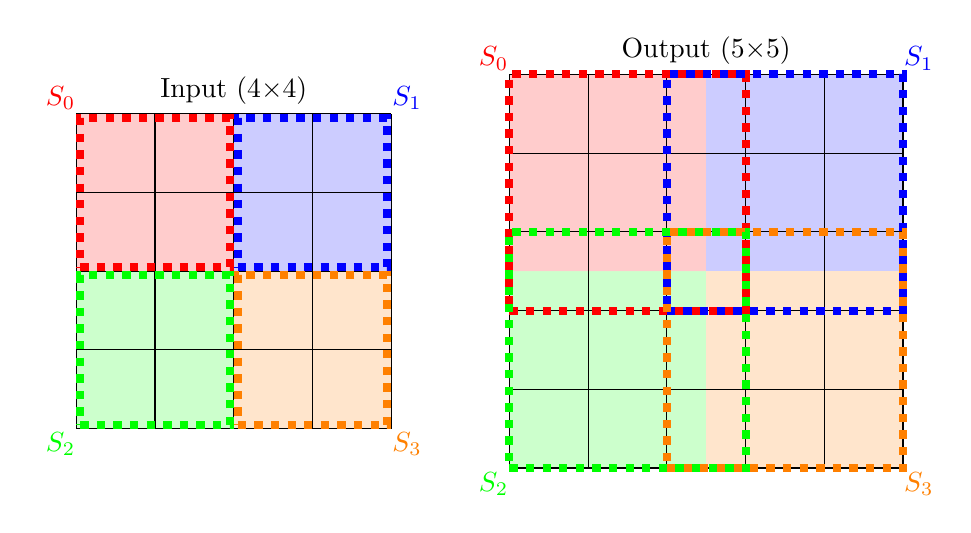
\begin{tikzpicture}%
  % Input
  \node (in) at (0,0) {};

  \path
    (in) --++ (0:1.5) --++ (90:3.5)
    node[
      fill=red!20,
      minimum width=2cm,
      minimum height=2cm
    ] {}
    
    --++ (0:2)
    node[
      fill=blue!20,
      minimum width=2cm,
      minimum height=2cm
    ] {}

    --++ (270:2)
    node[
      fill=orange!20,
      minimum width=2cm,
      minimum height=2cm
    ] {}

    --++ (180:2)
    node[
      fill=green!20,
      minimum width=2cm,
      minimum height=2cm
    ] {};

  \node[
    text=black,
    above,
    xshift=2.5cm,
    yshift=4.5cm
  ] at (in) {Input (4$\times$4)};

  \draw[
    step=1.0,
    black,
    thin
  ] let
      \p1=(in)
    in
      (in) grid[xshift=0.5cm,yshift=0.5cm] (\x1 + 4 cm,\y1 + 4 cm);

  \path
    (in) --++ (0:1.5) --++ (90:3.5)
    node[
      rectangle,
      draw=red,
      dashed,
      line width = 1 mm,
      minimum width=1.9cm,
      minimum height=1.9cm
    ] {} coordinate (is0)

    --++ (0:2)
    node[
      rectangle,
      draw=blue,
      dashed,
      line width = 1 mm,
      minimum width=1.9cm,
      minimum height=1.9cm
    ] {} coordinate (is1)

    --++ (270:2)
    node[
      rectangle,
      draw=orange,
      dashed,
      line width = 1 mm,
      minimum width=1.9cm,
      minimum height=1.9cm
    ] {} coordinate (is3)

    --++ (180:2)
    node[
      rectangle,
      draw=green,
      dashed,
      line width = 1 mm,
      minimum width=1.9cm,
      minimum height=1.9cm
    ] {} coordinate (is2);

  \node[
    text=red,
    xshift = -1.2cm,
    yshift = 1.2cm
  ] at (is0) {$S_0$};

  \node[
    text=blue,
    xshift = 1.2cm,
    yshift = 1.2cm
  ] at (is1) {$S_1$};

  \node[
    text=green,
    xshift = -1.2cm,
    yshift = -1.2cm
  ] at (is2) {$S_2$};

  \node[
    text=orange,
    xshift = 1.2cm,
    yshift = -1.2cm
  ] at (is3) {$S_3$};

  % Output
  \node (out) at (6,0) {};

  \node[
    text=black,
    above,
    xshift=2.5cm,
    yshift=5cm
  ] at (out) {Output (5$\times$5)};

  \fill[red!20]
    (out) --++ (90:5) coordinate (red) --++ (0:2.5) --++ (270:2.5) --++ (180:2.5);
  \fill[blue!20]
    (red) --++ (0:2.5) --++ (0:2.5) --++ (270:2.5) --++ (180:2.5) --++ (90:2.5);
  \fill[green!20]
    (out) --++ (90:2.5) coordinate (green) --++ (0:2.5) --++ (270:2.5) --++ (180:2.5);
  \fill[orange!20]
    (green) --++ (0:2.5) --++ (0:2.5) --++ (270:2.5) --++ (180:2.5) --++ (90:2.5);

  \draw[
    step=1.0,
    black,
    thin
  ] let
      \p1=(out)
    in
      (out) grid (\x1 + 5 cm,\y1 + 5 cm);

  \path
    (out) --++ (0:1.5) --++ (90:3.5)
    node[
      rectangle,
      draw=red,
      dashed,
      line width = 1 mm,
      minimum width=3cm,
      minimum height=3cm
    ] {} coordinate (os0)

    --++ (0:2)
    node[
      rectangle,
      draw=blue,
      dashed,
      line width = 1 mm,
      minimum width=3cm,
      minimum height=3cm
    ] {} coordinate (os1)

    --++ (270:2)
    node[
      rectangle,
      draw=orange,
      dashed,
      line width = 1 mm,
      minimum width=3cm,
      minimum height=3cm
    ] {} coordinate (os3)

    --++ (180:2)
    node[
      rectangle,
      draw=green,
      dashed,
      line width = 1 mm,
      minimum width=3cm,
      minimum height=3cm
    ] {} coordinate (os2);

  \node[
    text=red,
    xshift = -1.7cm,
    yshift = 1.7cm
  ] at (os0) {$S_0$};

  \node[
    text=blue,
    xshift = 1.7cm,
    yshift = 1.7cm
  ] at (os1) {$S_1$};

  \node[
    text=green,
    xshift = -1.7cm,
    yshift = -1.7cm
  ] at (os2) {$S_2$};

  \node[
    text=orange,
    xshift = 1.7cm,
    yshift = -1.7cm
  ] at (os3) {$S_3$};

\end{tikzpicture}
\end{document}
\end{filecontents*}

\begin{document}
  \input{plot}
  \input{matrix}
  \input{unit_circle}
  \input{fft}
  \input{pipeline}
  \input{oa}
\end{document}